% Multiple Choice Question 16

\begin{center}
    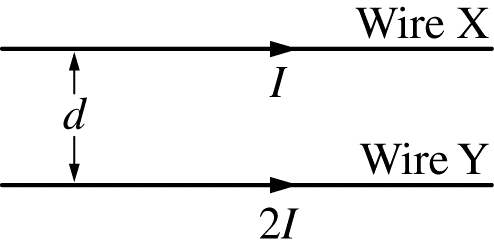
\includegraphics[scale=0.3]{images/img-009-017.png}
\end{center}

\begin{questions}
\setcounter{question}{15}
\question
Two long, straight parallel wires X and Y are separated by a distance $d$ and carry currents $I$ and $2 I$, as shown in the figure above. The force on wire X has magnitude $F$. If the current in each wire is both doubled and reversed in direction. which of the following is true of the magnitude and direction of the new force on wire X?

\tabto{0.75cm}\underline{Magnitude}
\tabto{3.00cm}\underline{Direction}

\begin{choices}
    \choice $F$   \tabto{2.25cm} Unchanged
    \choice $2 F$ \tabto{2.25cm} Reversed
    \choice $2 F$ \tabto{2.25cm} Unchanged
    \choice $4 F$ \tabto{2.25cm} Reversed
    \choice 4$ F$ \tabto{2.25cm} Unchanged
\end{choices}
\end{questions}
